\documentclass[11pt]{article}
\usepackage[a4paper,margin=2cm]{geometry}
\usepackage{graphicx,booktabs,amsmath,float,caption}
\usepackage[hidelinks]{hyperref}
\setlength{\parskip}{4pt}\setlength{\parindent}{0pt}

\title{\textbf{PRML Lab 3 --- Bagging \& Boosting}}
\author{Aryan Tiwari (B20AI056)\\CSL2050 Pattern Recognition \& Machine Learning, Winter 2022}
\date{}

\begin{document}
\maketitle

\textbf{Implementation note.} For Q1 tasks 1--8 and Q2 tasks 1--3 I wrote a CART decision tree from scratch.
It handles both regression (the split minimises the children's summed squared error; leaves predict the mean) and
classification (the split minimises weighted Gini impurity; leaves predict the majority class). At each node every
feature is sorted once and all thresholds are scored in one pass with cumulative sums. Random Forest,
AdaBoost, XGBoost and LightGBM come from their libraries, as the assignment allows.

\section*{Question 1 --- Housing prices (regression)}

\textbf{Pre-processing.} 545 houses, 12 features, no missing values or duplicates. The six yes/no columns were
mapped to 0/1 and \texttt{furnishingstatus} was encoded as an ordinal variable (unfurnished $<$ semi $<$ furnished). Price was
converted to lakhs so that errors are easy to read. Feature scaling is unnecessary because tree splits are unaffected by
monotonic transformations. 80:20 split: \texttt{Xtrain} = 436 rows, test = 109 rows.

\begin{figure}[H]\centering
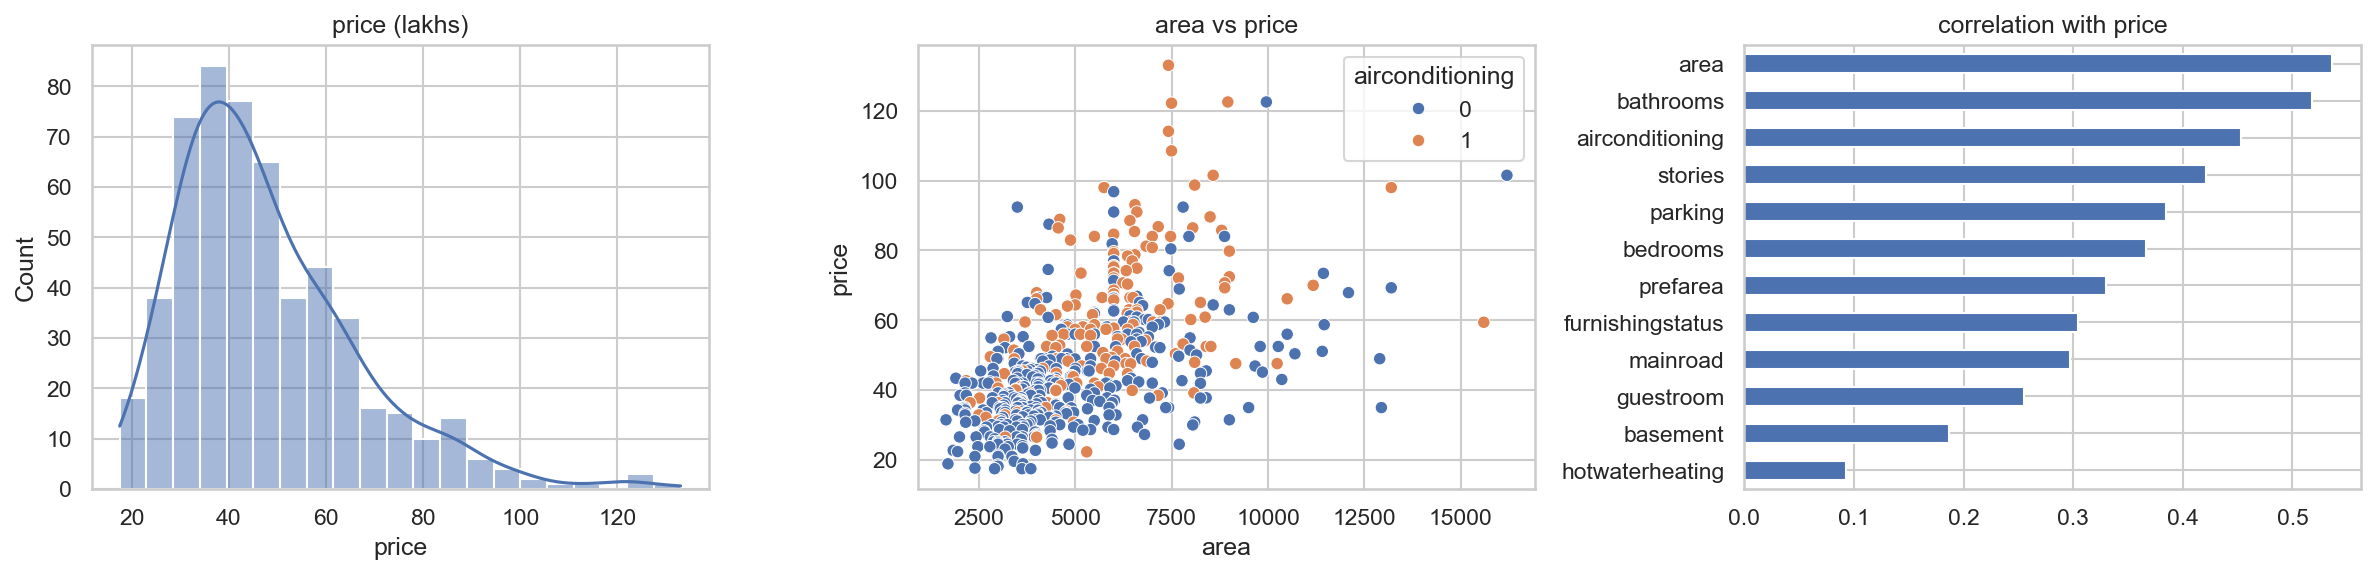
\includegraphics[width=\linewidth]{figures/q1_eda.png}
\caption{Price is right-skewed; area, bathrooms and air-conditioning correlate most with price.}
\end{figure}

\textbf{1. Single tree without validation.} A fully-grown tree reaches R$^2$ = 0.999 on the training data but only
\textbf{0.421} on the test set. It memorises the training data (the train R$^2$ falls just short of 1 because a few houses have identical
features but different prices) and generalises poorly, which is the high-variance problem that motivates bagging.

\textbf{2--3. 5-fold CV for \texttt{max\_depth}.} Mean validation R$^2$ peaks at \textbf{depth 3 (0.461 $\pm$ 0.120)}.
Shallower trees underfit. Deeper trees overfit: by depth 10 the mean drops to 0.25. The spread between folds is large
(fold 3 is the easiest at every depth, while folds 1 and 2 are the hardest), so a single train/validation split would have given an unreliable choice of depth.

\begin{figure}[H]\centering
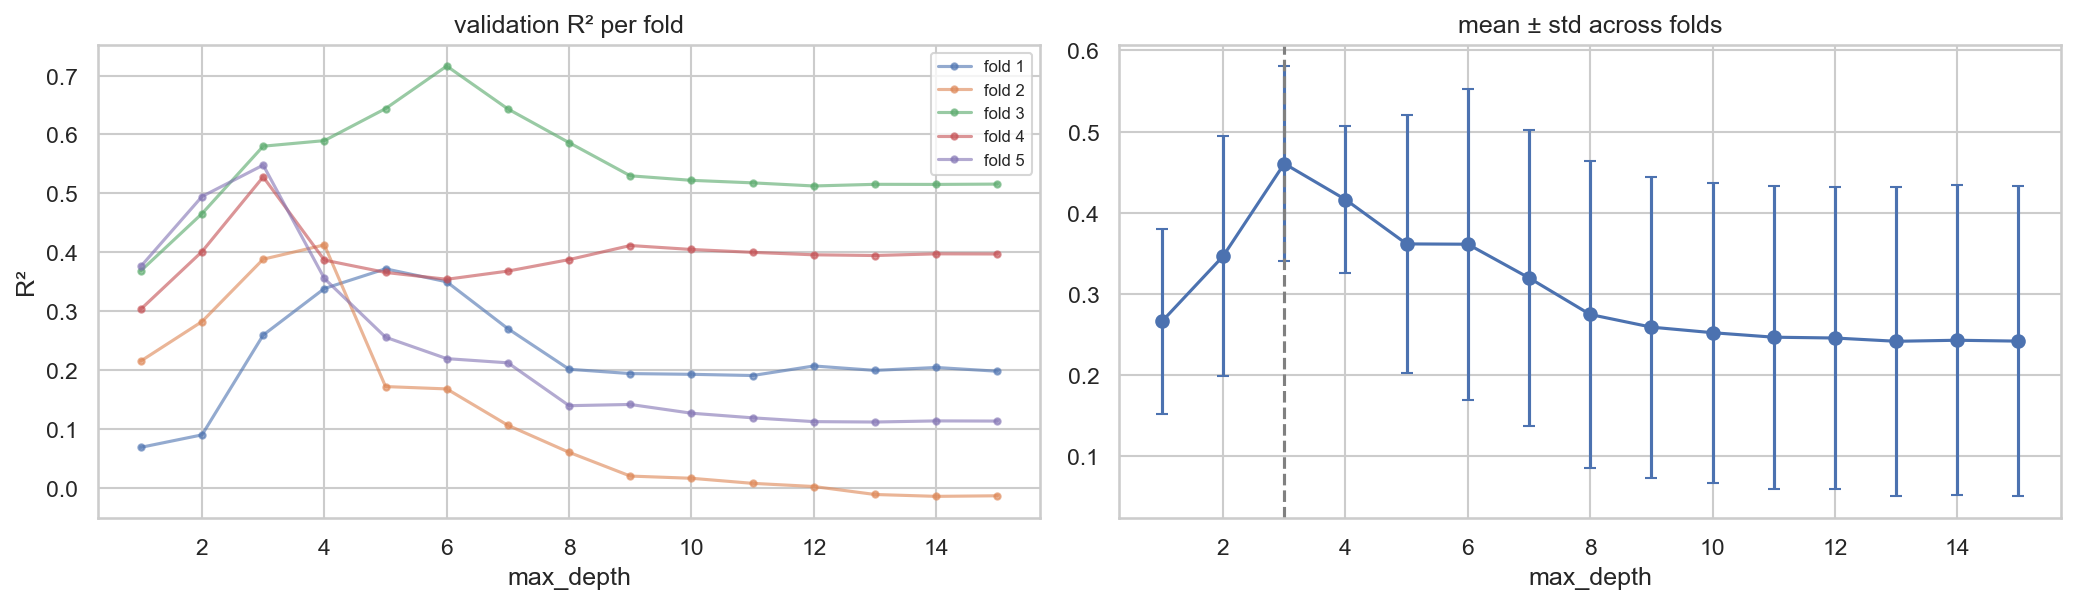
\includegraphics[width=\linewidth]{figures/q1_cv_depth.png}
\caption{Validation R$^2$ for each fold (left) and mean $\pm$ std (right).}
\end{figure}

\textbf{4--7. Bagging.} I drew ten bootstrap samples (each the size of \texttt{Xtrain}, drawn with replacement, so about 63\% of
rows are unique) and trained one depth-3 tree on each. On the test set the individual trees score R$^2$ between
0.349 and 0.481, averaging \textbf{0.425 $\pm$ 0.041}. Averaging their predictions gives
\textbf{R$^2$ = 0.524} --- better than every single tree. Averaging cancels the parts of each tree's errors that
are not shared with the others, so variance falls while bias stays the same.

\begin{figure}[H]\centering
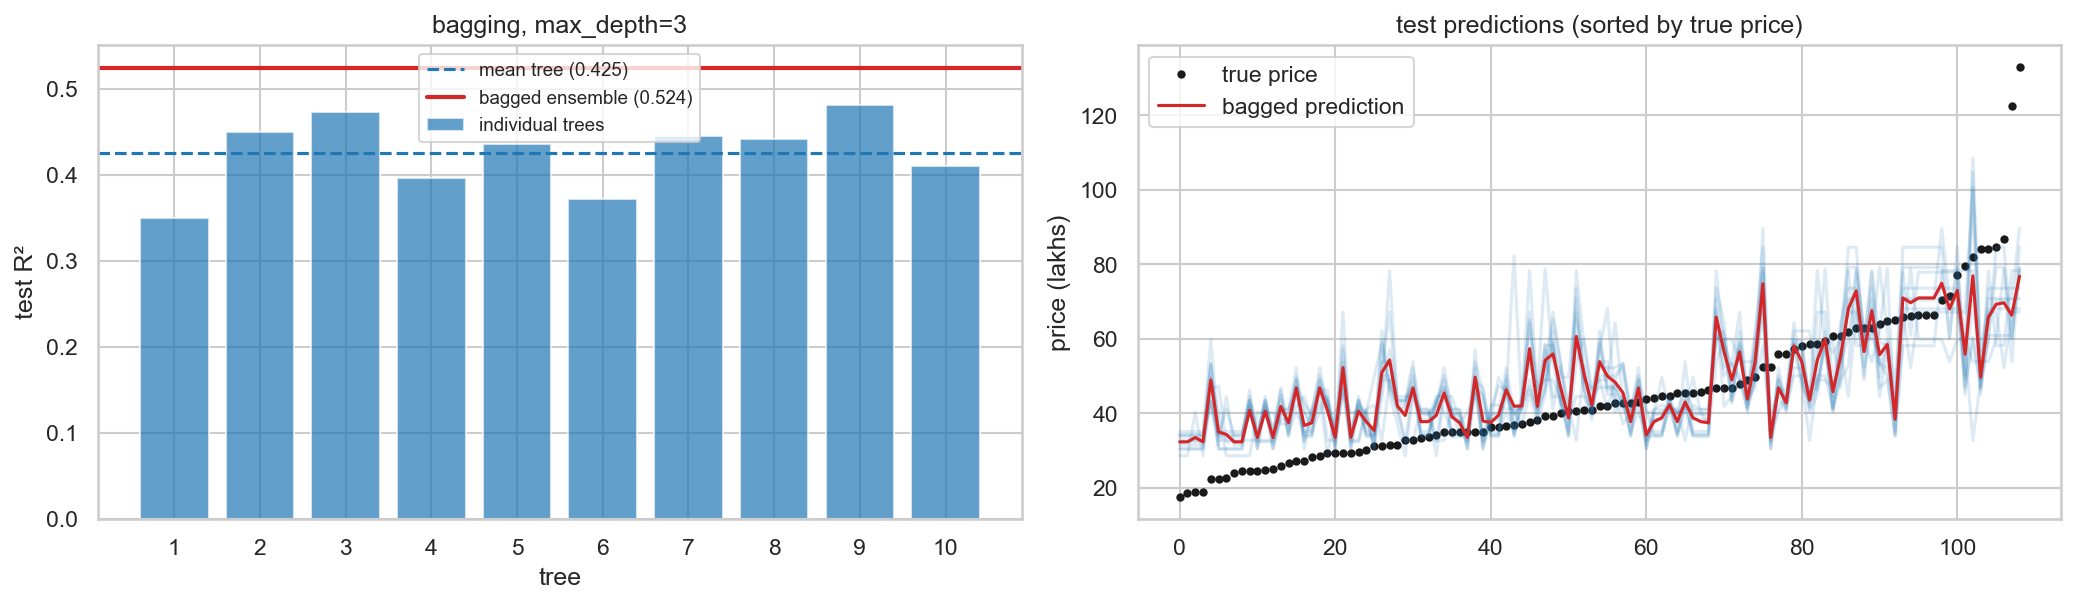
\includegraphics[width=\linewidth]{figures/q1_bagging.png}
\caption{Per-tree vs.\ bagged R$^2$ (left); the bagged prediction (red) is a smoothed version of the 10 trees (blue).}
\end{figure}

\textbf{8. Changing \texttt{max\_depth}.} The gain from bagging grows with depth: +0.03 R$^2$ at depth 1, +0.10 at depth 3,
+0.25 at depth 8 and +0.28 for unlimited depth. Deep trees have low bias and high variance, which is exactly what averaging removes,
so the bagged R$^2$ \emph{rises} to about 0.62 even though each deep tree on its own gets \emph{worse} (0.34).
Shallow trees have high bias and low variance, and averaging cannot fix bias. So when bagging, you should grow deep trees, not the depth that is
optimal for a single tree.

\begin{figure}[H]\centering
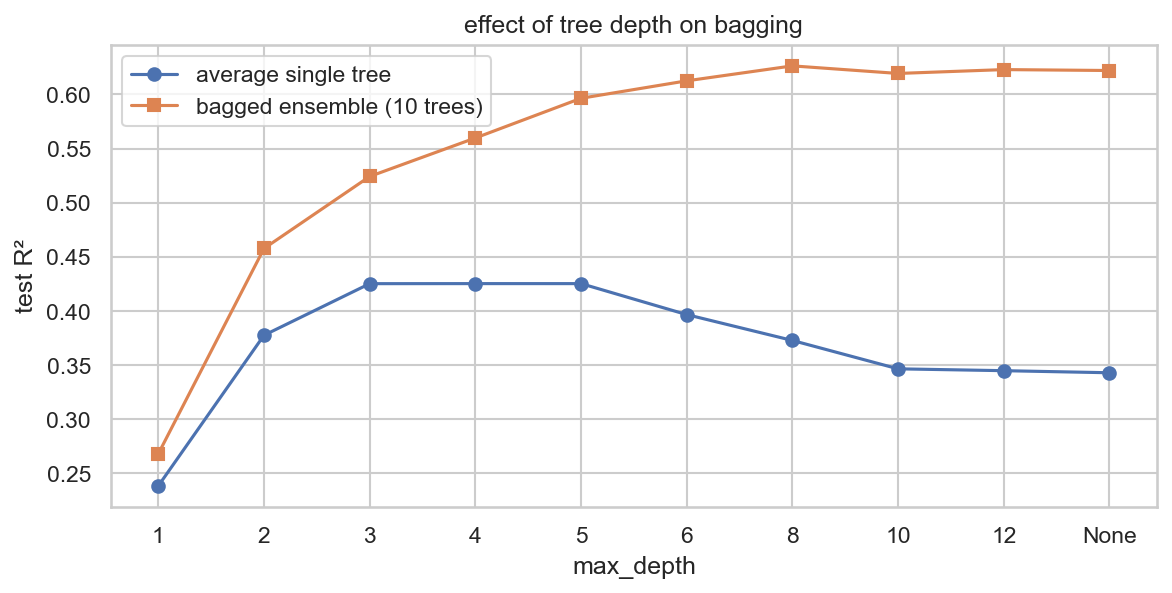
\includegraphics[width=0.65\linewidth]{figures/q1_depth_bagging.png}
\caption{Average single-tree vs.\ bagged test R$^2$ as tree depth increases.}
\end{figure}

\textbf{9--10. Random Forest and AdaBoost.}
\begin{table}[H]\centering
\begin{tabular}{lccc}\toprule
Model (test set) & MSE (lakh$^2$) & MAE (lakh) & R$^2$\\\midrule
Single tree, depth 3 & 211.1 & 11.00 & 0.480\\
Bagging, 10 trees (scratch) & 193.1 & 10.50 & 0.524\\
Random Forest, 200 trees & \textbf{140.2} & \textbf{8.37} & \textbf{0.655}\\
AdaBoost, 200 estimators & 178.5 & 10.20 & 0.560\\\bottomrule
\end{tabular}
\end{table}
Random Forest is clearly best. It uses deep trees, many more of them, and random feature subsets at each split,
which makes the trees less correlated, so averaging reduces variance more than plain bagging does. AdaBoost improves on a
single tree by focusing successive learners on the houses with the largest errors, but price has heavy-tailed noise and that
limits it.

\section*{Question 2 --- Breast cancer (classification)}

569 samples, 5 numeric features, labels 357 / 212, no missing values. Radius, perimeter and area are almost
perfectly correlated (all three measure size). 80:20 stratified split (455 / 114).

\textbf{1. Single fully-grown tree.} Train accuracy 100\%, test accuracy \textbf{91.2\%}.

\textbf{2--3. 5-fold CV for \texttt{max\_depth}.} Mean validation accuracy is highest at \textbf{depth 5 (89.9\% $\pm$ 1.6\%)};
refitting at that depth raises test accuracy to \textbf{94.7\%}, compared with 91.2\% for the unpruned tree. The CV curve is fairly flat
(87--90\%), because a single split on size already separates most cases.

\begin{figure}[H]\centering
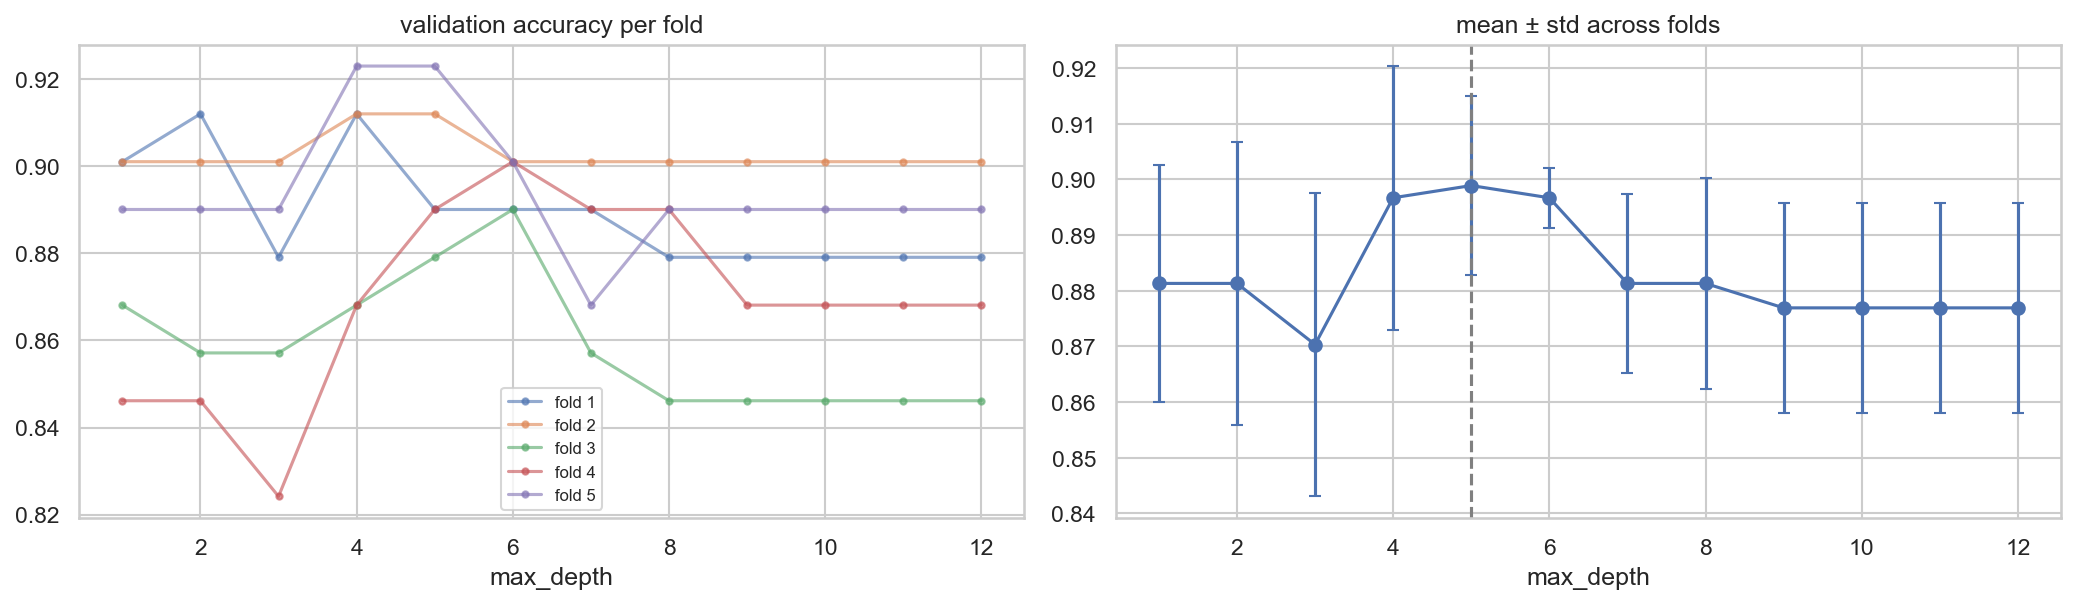
\includegraphics[width=\linewidth]{figures/q2_cv_depth.png}
\caption{Validation accuracy per fold and mean $\pm$ std for the scratch classifier.}
\end{figure}

\textbf{4--5. XGBoost} (\texttt{subsample}=0.7, \texttt{max\_depth}=4, 200 rounds): train accuracy 100\%, test accuracy \textbf{95.6\%}.
Row subsampling makes each boosting round see a different 70\% of the data, which acts like bagging inside boosting.

\textbf{6--7. LightGBM, \texttt{max\_depth} vs.\ \texttt{num\_leaves}.} A tree of depth $d$ has at most $2^d$ leaves, so with
\texttt{max\_depth}=3 any \texttt{num\_leaves} $>8$ has no effect: every metric is identical from 8 leaves up. LightGBM grows trees
\emph{leaf-wise}, so \texttt{num\_leaves} is its main complexity control and \texttt{max\_depth} is a cap on top of it.
On a 114-sample test set accuracy only moves in steps of 0.9\%, so I also tracked log-loss:

\begin{table}[H]\centering
\begin{tabular}{lcccccc}\toprule
\texttt{num\_leaves} & 2 & 3 & 4 & 6 & 8 & 16\\\midrule
test log-loss, depth 3 & 0.120 & \textbf{0.106} & 0.107 & 0.114 & 0.144 & 0.144\\
test log-loss, no depth limit & 0.120 & \textbf{0.106} & 0.107 & 0.117 & 0.144 & 0.248\\
train log-loss, no depth limit & 0.121 & 0.062 & 0.031 & 0.009 & 0.002 & 0.000\\\bottomrule
\end{tabular}
\end{table}

Test loss is lowest at 3--4 leaves. \textbf{Overfitting starts at about 6 leaves}: train loss keeps falling towards zero while
test loss rises. Without a depth cap it more than doubles by 16 leaves (0.248). In accuracy terms, train accuracy reaches
100\% as soon as \texttt{num\_leaves} $\ge 4$ (with depth $\ge 3$) while test accuracy stays at about 95--96\%.

\begin{figure}[H]\centering
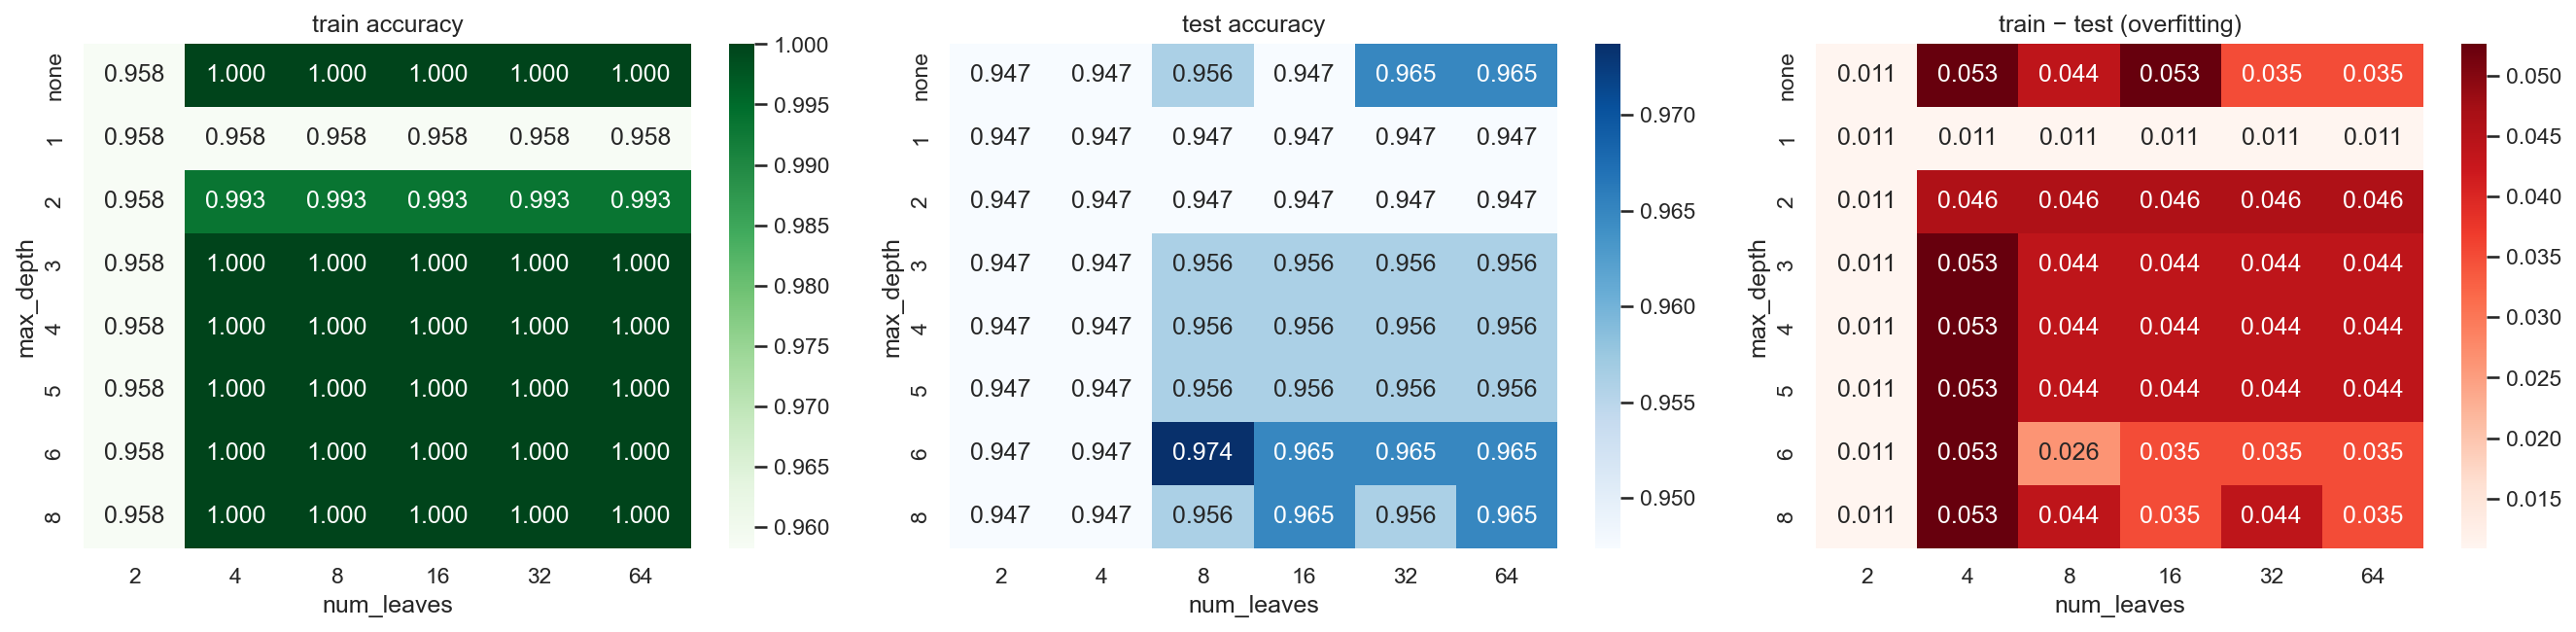
\includegraphics[width=\linewidth]{figures/q2_lgbm_grid.png}
\caption{Train accuracy, test accuracy and their gap over \texttt{max\_depth} $\times$ \texttt{num\_leaves} (none = no limit).}
\end{figure}

\begin{figure}[H]\centering
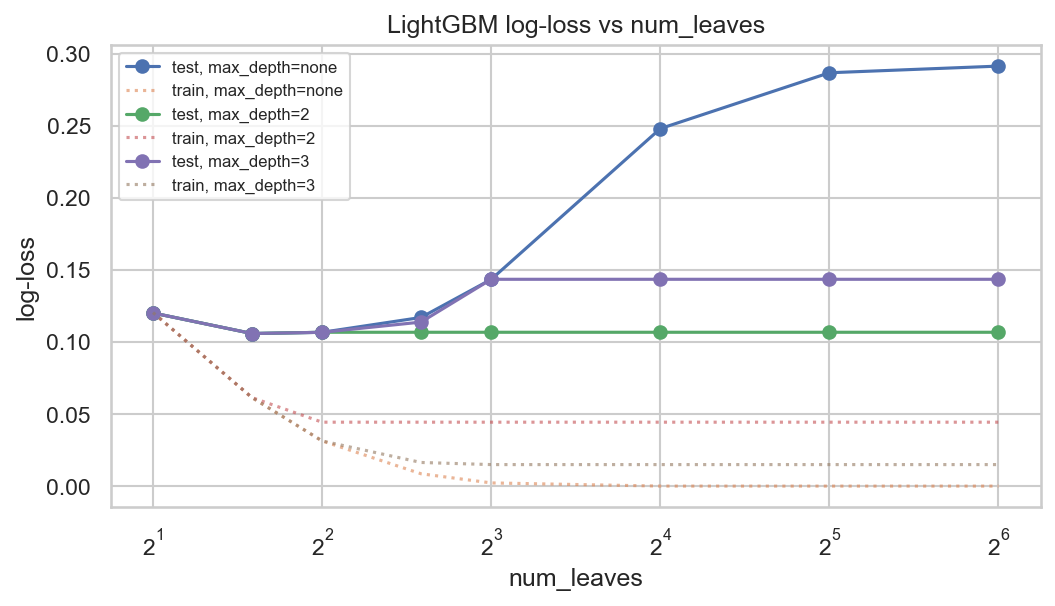
\includegraphics[width=0.6\linewidth]{figures/q2_lgbm_logloss.png}
\caption{Log-loss vs.\ \texttt{num\_leaves}; dotted lines are training loss.}
\end{figure}

\textbf{8. Parameters for accuracy vs.\ overfitting.}
\begin{itemize}\itemsep0pt
\item \emph{More capacity / accuracy:} \texttt{num\_leaves}, \texttt{max\_depth}, \texttt{n\_estimators} together with a smaller \texttt{learning\_rate}.
These help until the model starts fitting noise.
\item \emph{Controlling overfitting:} keep \texttt{num\_leaves} below $2^{\texttt{max\_depth}}$; raise \texttt{min\_child\_samples}
(minimum data in a leaf); use row and feature subsampling (\texttt{bagging\_fraction}/\texttt{subsample},
\texttt{feature\_fraction}/\texttt{colsample\_bytree}); use L1/L2 regularisation (\texttt{lambda\_l1}, \texttt{lambda\_l2});
and use early stopping on a validation set.
\end{itemize}
On this dataset a very small model (3--4 leaves) generalises best, because the classes are almost separable by tumour size.

\end{document}
